\subsection{Armazenamento}

	Neste projeto será utilizada a câmera Waveshare OV5647 Night Vision. É uma câmera já voltada para sistemas de vigilância, muito utilizada em escritórios e shoppings.

	Serão utilizadas, no total, 15 câmeras do modelo  Waveshare ov5647, e para conseguir armazenar os videos gravados utilizaremos o HD Seagate Archive 8TB. Como o sistema funcionará  24x7, ou seja, 24 horas por 7 dias da semana, o servidor irá passar as imagens caso a situação seja considerada de risco, as imagens irão para o HD a uma taxa de 1024 Kbps, em um mês (considerando um mês como 30 dias), será gasto um total de 4.63TB.

\begin{table}[H]
	\centering
	\begin{tabular}{|l|l|}
		\hline
		Capacidade                  & 8TB            \\ \hline
		Modelo                      & ST8000AS0002    \\ \hline
		Interface                   & SATA de 6 GB/s \\ \hline
		Velocidade da rotação       & 5900 RPM       \\ \hline
		Cache                       & 128 MB          \\ \hline
		Impacto máximo de operação  & 80 Gs          \\ \hline
		Tipo de armazenamento       & HDD            \\ \hline
		Comprimento                 & 147.00 mm      \\ \hline
		Largura                     & 101.85 mm      \\ \hline
		Altura                      & 26.1 mm        \\ \hline
		Peso típico                 & 795 g          \\ \hline
		AFR                         & 0.55\%         \\ \hline
		Potência média de operação  & 7.500 W        \\ \hline
		Taxa de transferência       & 600 MB/s       \\ \hline
		Taxa de dados sustentada DE & 180            \\ \hline
	\end{tabular}
	\caption[Especificações da Seagate Archive 8TB]{Especificações da Seagate$^{\textregistered}$ Archive 8TB~\cite{seagate}}
	\label{my-label}
\end{table}

\begin{table}[H]
\centering
\begin{tabular}{|p{5cm}|p{10cm}|}
\hline
Processador              & Intel Core i7 - 4700K                                                   \\ \hline
Placa-mãe                & ASRock Z87Killer                                                        \\ \hline
Memoria                  & 16 GB G. Skill Spiner (DDR 3 - 1600/PC3 - 12800), configurada a 1600MHz \\ \hline
Placa de vídeo           & GeForce GT 630 1GB                                                      \\ \hline
Resolução de vídeo       & 1920x1080                                                               \\ \hline
Fonte de alimentação     & Corsair CX500M                                                          \\ \hline
Unidade de inicialização & Kingston HyperX 3k 480 GB                                               \\ \hline
\end{tabular}
\caption{Configuração de Hardware}
\label{tab:configHardware}
\end{table}

Em tempos de muitas chuvas, ocorre uma grande variação de energia, devido às descargas
elétricas de raios. Para que não se tenha o problema de o sistema parar de funcionar por falta de
energia, e pela variação de energia, não chegar a queimar o sistema ou danificar o sistema,
será utilizado um equipamento que armazenar energia por algum tempo.

O equipamento utilizado para o sistema de energia nobreak, será o \textbf{Nobreak Organizador e
Fonte para 16 câmeras}, da tecnologia ONAT. Com este equipamento, o armazenamento de
dados terá em média 4 horas de autonomia, ou seja, caso por algum motivo a luz acabe o
sistema terá em média 4 horas funcionando perfeitamente \cite{nobreak}.

O Seagate para gravação e backup de imagens deverá ser alimentado pelo sistema de energia
(nobreak), de forma a possibilitar a operação em caso de falta de energia elétrica.

\begin{table}[H]
\centering
\begin{tabular}{|l|l|l|l|}
\hline
                      & Unidades & Preço de uma unidade & Preço total    \\ \hline
Waveshare OV5647 Night Vision   & 15       & R\$ 123,34         & R\$ 1850,10 \\ \hline
Seagate$^{\textregistered}$ Vídeo 3.5 HDD & 4        & R\$ 984,90           & R\$ 3.939,60   \\ \hline
Sistema Nobreak       & 1        & R\$ 396,90           & R\$ 396,90      \\ \hline
Hardware              & 1        & R\$ 5.271,86         & R\$ 5.271,86    \\ \hline
\multicolumn{4}{|r|}{R\$ 11.458,46}                                     \\ \hline
\end{tabular}
\caption{Tabela de preços}
\label{table:precosComponentes}
\end{table}

\subsection{Comunicação da estação de solo com a segurança}

O sistema de comunicação será dado de maneira manual, ou seja, terá uma pessoa na estação de solo que será responsável por analisar os monitores de vigilância que  informam as áreas de possíveis situações de risco mediante a pontuação preestabelecida no sistema. E caso seja necessário, o operador irá alertar um segurança para que ele possa averiguar tal situação. O sistema será uma ferramenta para o operador, auxiliando e facilitando o monitoramento do estacionamento.

Essa comunicação será dada via voz, utilizando um rádio comunicador, ou walk talk. Este meio de comunicação é bem utilizado em sistemas de vigilância de escritórios, shoppings, em construções civis ou em operações de policiais e bombeiros.

Os Walkie Talkies tem um alcance relativamente alto, exatamente o necessário para suprir a carência de sinal de celular presente na área da FGA, e este equipamento terá um alcance de  56km. Neste sistema de monitoramento será utilizado o rádio comunicador walk talk Cobra Cxr925 56km.

\begin{table}[H]
\centering
\begin{tabular}{|l|l|}
\hline
Peso        & 68g                          \\ \hline
Alcance     & 56 km                        \\ \hline
Dimensões   & 177,50mm x 49,00mm x 33,00mm \\ \hline
Frequência  & 22 canais                    \\ \hline
Alimentação & 110 V                        \\ \hline
Preço       & R\$ 415,99                   \\ \hline
\end{tabular}
\caption[Especificações e preço do Walk Talk Cobra Cxr925 56km]{Especificações e preço do Walk Talk Cobra Cxr925 56km~\cite{walk}}
\label{table:walk}
\end{table}

\subsection{Processamento dos dados}

Para o armazenamento se tornar eficiente e confiável, além de resiliente, será implementado o
padrão RAID(\textbf{Redundant Array of Independent Disks}) em seu nível um também conhecido por
Mirror.

Todas as informações vindas processadas para armazenamento serão copiadas
simultaneamente em dois HDs, reduzindo a performance porém mantendo assim a segurança,
pois caso haja algum problema técnico em um dos armazenamentos, não haverá nenhuma
perda de informação. Neste projeto serão utilizados 4 Seagate® Vídeo 3.5 HDD para o
armazenamento das imagens do monitoramento, formando 2 pares de HDs, que serão
redundantes \cite{raid}.

Cada par será capaz de armazenar informações por 30 dias, uma vez cheio as informações passarão a ser armazenadas no par ocioso, formando assim um total de 60 dias de armazenamento de informação, ao final deste período, informações armazenadas serão a ser eliminadas, sendo assim necessário realizar cópias para outros dispositivos caso seja necessário o uso em um período posterior.O tempo em média para recuperação das imagens será de uma a duas horas.

\subsubsection{Redundância de software}

Um software bem projetado corretamente desde a sua elaboração, não necessita de técnicas de tolerância para software, mesmo que ainda não seja possível garantir na pratica que todo programa estarão corretos \cite{webertolerancia}.

As formas usuais de redundância de software são:

\begin{itemize}
	\item Diversidade (ou programação n-versões)
	\item Blocos de recuperação
\end{itemize}

\paragraph{Diversidade}

Diversidade, também chamada programação diversitária, é uma técnica de redundância usada para obter tolerância a falhas em software. A partir de um problema a ser solucionado são implementadas diversas soluções alternativas, sendo a resposta do sistema determinada por votação.

Os erros,para poderem ser detectados, devem se manisfestar de forma diferente nas diversas alternativas, ou seja, devem ser estatisticamente independentes. Experimentalmente foi comprovado que o número de erros idênticos(erros que não seriam detectados) é consideravelmente menor que o número total de erros.

Diversidade pode ser utilizada em todas as fases de desenvolvimento do projeto. Essa técnica é chamada de projeto diversitário quando o desenvolvimento do sistema é ralizado de forma diversitároa e de programação em varias versões quando se restringe á implementação do sistema.

Os pontos negativos dessa técnica devem ser colocadas em pauta, como o aumento dos custos de desenvolvimento e manutenção, a complexidade de sincronização das veres e o problema de determinar a correlação das fontes de erro.

\paragraph{Blocos de recuperação}

Nessa técnica programas secundários só serão necessários na detecção de um erro no programa primário.Essa estratégia envolve um teste de aceitação.Programas são executados e testados um a um até que o primeiro passa no teste de aceitação. A estratégia de blocos de recuperação tolera n-1 falhas, no caso de falhas independentes nas n versões.

\begin{figure}[H]
	\centering
	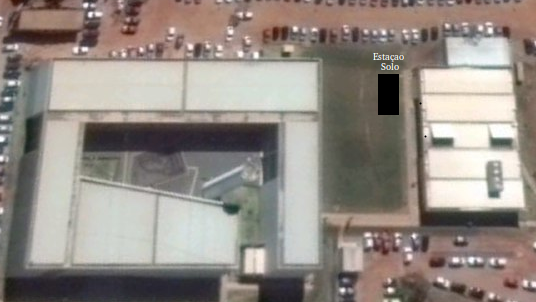
\includegraphics[width=0.6\textwidth]{figuras/estacaoSolo}
	\caption{Local da Estação Solo}
	\label{img:estacaoSoloLocal}
\end{figure}

\textbf{Diagrama de Caso de Uso}

\begin{figure}[H]
	\centering
	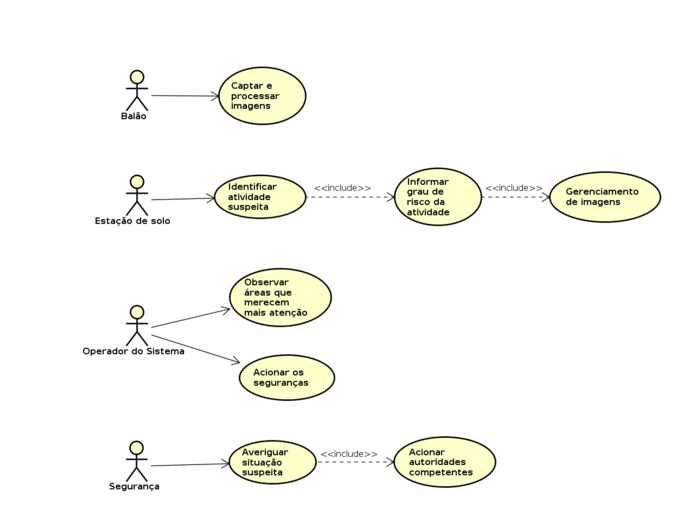
\includegraphics[width=0.7\textwidth]{figuras/Casosdeuso}
	\caption{Diagrama de Caso de Uso}
	\label{img:Casos de Uso}
\end{figure}

\textbf{Operacionabilidade do Sistema}

\begin{figure}[H]
	\centering
	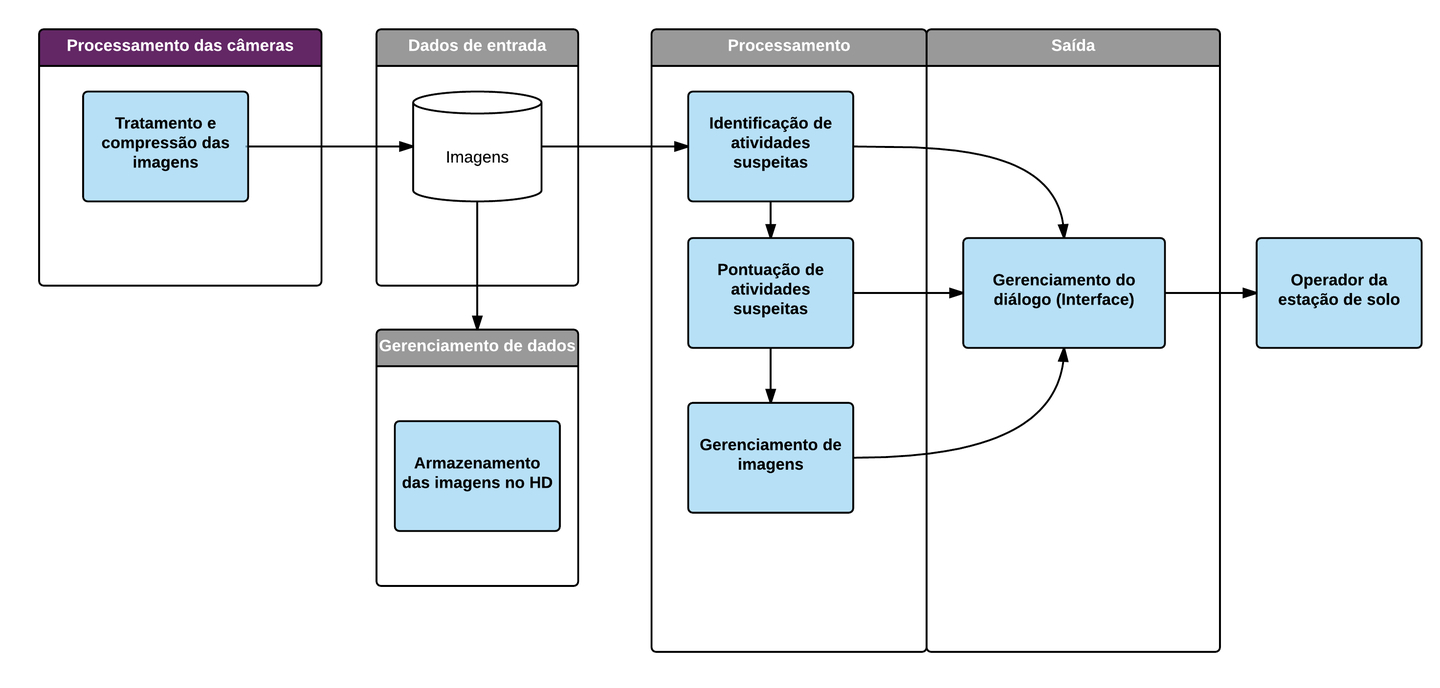
\includegraphics[width=1\textwidth]{figuras/OperacionabilidadedoSistema}
	\caption{Diagrama de Arquitetura: Operacionalibilidade do Sistema}
	\label{img:Operacionabilidade do Sistema}
\end{figure}

O sistema funcionará da seguinte maneira: no balão ocorrerá o processamento e tratamento das imagens recebidas (Processamento das câmeras). Após serem tratadas, estas imagens serão armazenadas em um HD da estação de solo(Gerenciamento de dados).

Em outro processo paralelo, estas imagens  irão fornecer os dados para que o sistema execute suas funcionalidades, como o gerenciamento das imagens, a identificação e pontuação das situações de risco (Processamento). E a saída do sistema será por meio de uma interface que interagirá com o operador da estação de solo.

\subsection{Processo de Monitoramento}
O processo de monitoramento do Sistema Unificado de Monitoramento (SUM), relativo ao modus operandi dos agentes do sistema, é ilustrado pelo diagrama a seguir:

\begin{figure}[H]
\centering
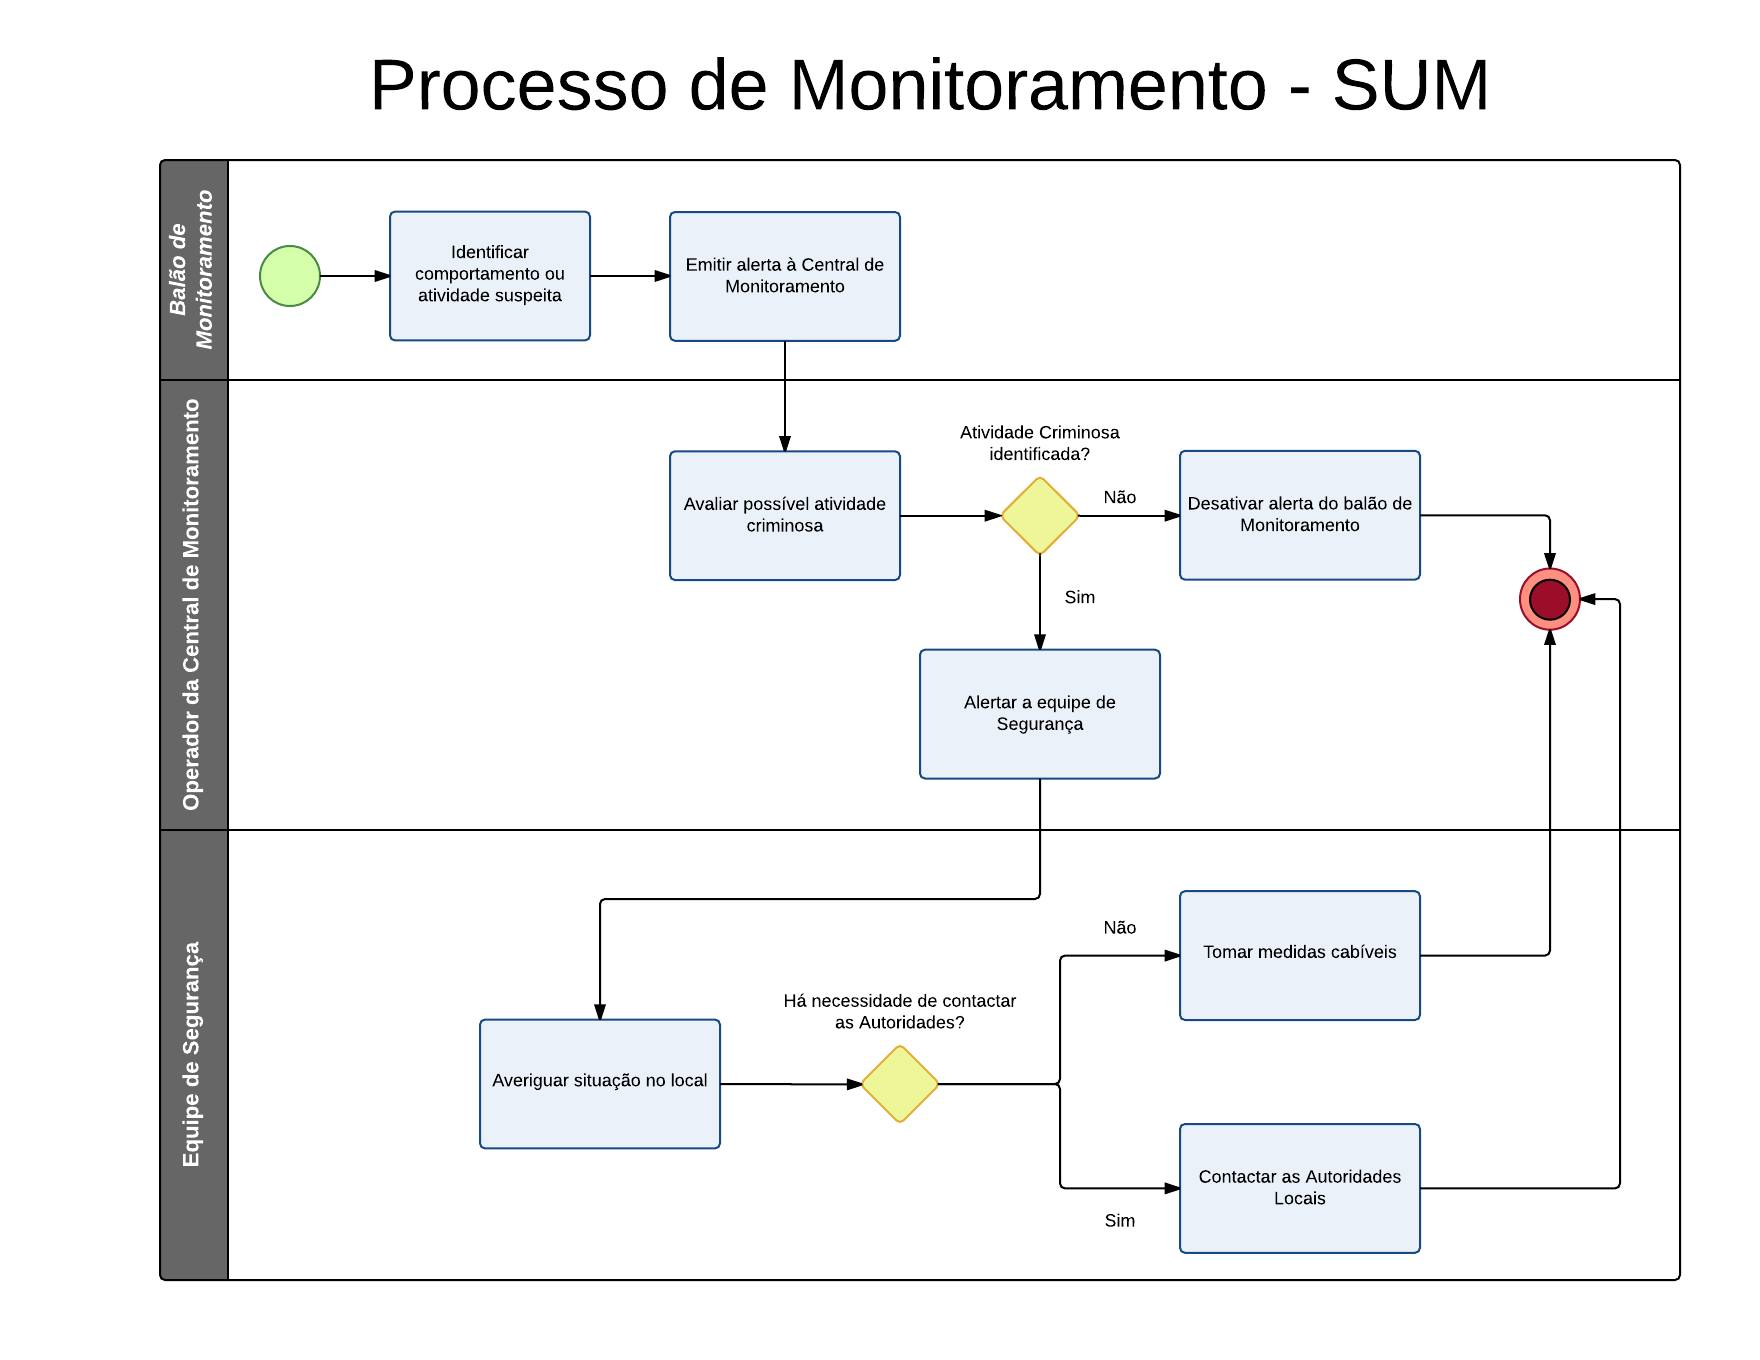
\includegraphics[width=0.9\textwidth]{figuras/Processodemonitorament}
\caption{Processo de Monitoramento}
\label{img:Processo de Monitoramento}
\end{figure}
As atividades contempladas neste processo estão descritas abaixo:
\\

\textbf{Identificar comportamento ou atividade suspeita} - O processo é iniciado a partir da identificação de comportamento ou atividade suspeita por parte do balão de monitoramento, que leva em consideração fatores de risco que determinam se uma atividade é normal, duvidosa ou suspeita.
\\

\textbf{Emitir alerta à central de Monitoramento} - Nesta atividade o sistema do balão, após ter identificado uma atividade suspeita nas dependências do estacionamento, emiti um sinal de alerta à Central de monitoramento contatando o operador do sistema.
\\

\textbf{Avaliar possível atividade criminosa} - Nesta atividade o operador do sistema, após ter sido notificado pelo balão sobre uma atividade suspeita, acompanhará através das câmeras de vídeo do balão , em tempo real, a ação do suspeito, avaliando se esta é uma atividade criminosa.
\\

\textbf{Desativar alerta do balão de monitoramento} - Nesta atividade o operador do sistema, após ter recebido e avaliado o alerta de atividade suspeita emitido pelo balão e concluído que este não retrata uma atividade criminosa, desativará o alerta do balão para aquela ação em específico, encerrando o processo.
\\

\textbf{Alertar a equipe de Segurança} - Nesta atividade o operador do sistema, após ter concluído que o alerta do balão se trata de fato de uma atividade criminosa, irá contactar a equipe de Segurança em campo emitindo um alerta via rádio.
\\

\textbf{Averiguar a situação do local} - Nesta atividade a equipe de Segurança, após receber um alerta do operador do sistema sobre uma atividade criminosa, irá averiguar a situação , no local informado, para avaliar a possibilidade de intervenção e/ou impedimento da ação criminosa.
\\

\textbf{Tomar medidas cabíveis} - Nesta atividade a equipe de Segurança, após concluir que há possibilidade de intervenção e/ou impedimento da ação criminosa, tomará as medidas cabíveis para que o infrator seja detido, encerrando o processo.
\\

\textbf{Contactar as autoridades locais} - Nesta atividade a equipe de Segurança, após concluir que não há possibilidade de intervenção e/ou impedimento da ação criminosa por quaisquer razões, irá contactar as Autoridades locais responsáveis para que estes tomem as medidas cabíveis à situação.
\\
\par
\textbf{Requisitos do Sistema de Monitoramento}
\begin{table}[H]
\centering
\begin{tabular}{|l|l|}
\hline
\textbf{Sigla}        & \textbf{Descricao} \\ \hline
NEC     & Necessidade                      \\ \hline
CAR   	& Característica				   \\ \hline
UC  	& Casos de uso                     \\ \hline
RNF 	& Requisito Não-Funcional          \\ \hline

\end{tabular}
\caption{Requisitos do Sistema de Monitoramento}
\label{Requisitos do Sistema de Monitoramento}
\end{table}

\textbf{Necessidades}
\par
A partir do processo de monitoramento descrito no tópico acima abstraiu-se as necessidades dos agentes do sistema.

As necessidades são:
\begin{itemize}
	\item NEC01 - O operador do sistema precisa receber um alerta do sistema de monitoramento quando houver uma atividade suspeita ocorrendo no estacionamento.
	\item NEC02 - O operador do sistema precisa visualizar em tempo real a ação do suspeito através das câmeras do balão de monitoramento.
	\item NEC03 - O operador do sistema precisa conseguir aproximar a imagem de forma a ser possível enxergar detalhes da ação do suspeito.
	\item NEC04 - O operador do sistema precisa visualizar áreas específicas do estacionamento para acompanhar o que ocorre em cada setor.
\end{itemize}

\textbf{Características}
\par
As características deviradas a partir das necessidades dos agentes do sistema são:
\begin{itemize}
	\item CAR01 - O sistema irá prover alertas de atividade suspeita na interface do usuário.
	\item CAR02 - O sistema deve permitir que um alerta de atividade suspeita seja desativado.
	\item CAR03 - O sistema deve permitir o acesso às câmeras de vídeo do balão de monitoramento.
\end{itemize}
